\begin{frame}
\begin{table}[htbp]
\centering
\caption{F0 Scores of Random Models}
\begin{tabular}{cc}
\toprule
Model & F0 Score \\
\midrule
Model 1 & 0.75 \\
Model 2 & 0.68 \\
Model 3 & 0.82 \\
\bottomrule
\end{tabular}
\end{table}
\end{frame}

\begin{frame}
\begin{table}[htbp]
\centering
\caption{Multicolumn Table}
\begin{tabular}{ccccc}
\toprule
\multicolumn{2}{c}{Group 1} & \multicolumn{3}{c}{Group 2} \\
\cmidrule(r){1-2} \cmidrule(l){3-5}
A & B & C & D & E \\
\midrule
1 & 2 & 3 & 4 & 5 \\
6 & 7 & 8 & 9 & 10 \\
\bottomrule
\end{tabular}
\end{table}


\end{frame}
\begin{table}[htbp]
\centering
\caption{Multirow Table}
\begin{tabular}{ccc}
\toprule
\multirow{2}{*}{Group} & \multicolumn{2}{c}{Values} \\
\cmidrule(r){2-3}
 & A & B \\
\midrule
1 & 2 & 3 \\
\midrule
\multirow{2}{*}{2} & \multicolumn{1}{c}{4} & \multicolumn{1}{c}{5} \\
 & 6 & 7 \\
\bottomrule
\end{tabular}
\end{table}
\begin{frame}

\end{frame}
\begin{frame}{Tables}{Task-4}
    Try the task-4, the solution is...\\ \pause
    \vspace{1em}
    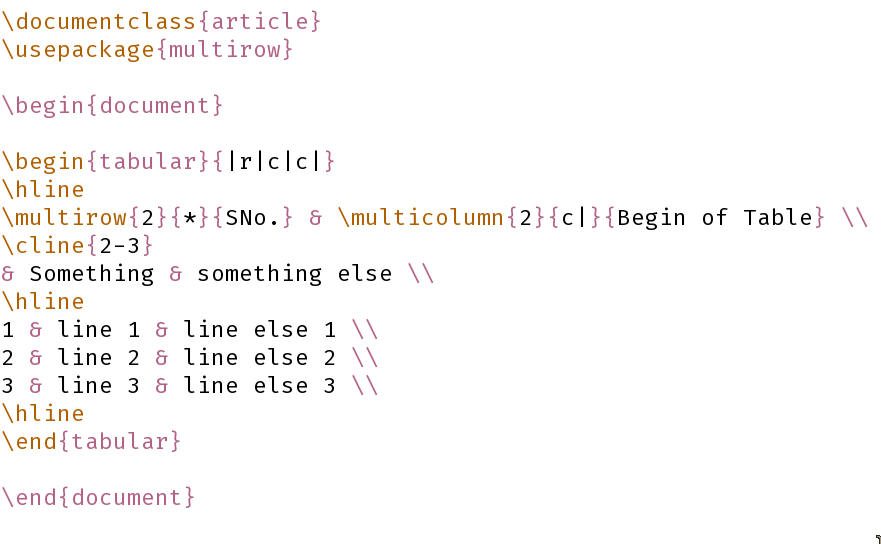
\includegraphics[width=0.8\textwidth]{4.png}
\end{frame}
